% Appendix 4: Axonometry
% Source pages: 257–260

\chapter{Axonometry}

\srcpage{257}

Axonometry is a special case of both the linear-perspective system and the perceptual
system.  For the first this is a well-known fact; for the second it follows at least from the
observation that for distant regions of space both perspective systems are geometrically
similar.  Let us examine the related questions in more detail.

To assess the degree of axonometric character of an image, introduce the quantity~$\Delta$,
defined as the relative change in width of an object with increasing depth (i.e.\ increasing
distance from the picture plane to that object).  Taking the road width from Appendix~3 as
the basis of the calculation, one can form two functions $\Delta$:
\begin{align}
  \Delta_1 &= (x_1' - x_1'')/x_1', \tag{4.1a} \\
  \Delta_2 &= (x_2' - x_2'')/x_2'. \tag{4.1b}
\end{align}
Here $x_1'$ and $x_2'$ are the road widths in the linear and perceptual perspective systems
respectively at distance~$l$ from the picture plane, and $x_1''$ and $x_2''$ are the same
widths at distance $l + \delta$ from the picture plane.  Thus the quantities $\Delta_1$ and
$\Delta_2$ characterise the degree of axonometric character of a region of depth~$\delta$
beginning at distance~$l$ from the picture plane.  In the case of ideal axonometry the road
width does not change with depth (i.e.\ $x'' = x'$), and for the function~$\Delta$ the
equality
\begin{equation}
  \Delta = 0 \tag{4.2}
\end{equation}
holds, which is the criterion of ideal axonometric character.  If $\Delta \neq 0$, the degree
of closeness to axonometry may be judged by how close $\Delta$ is to zero.

Based on formulas~(1.1) and~(1.3), one can write

\srcpage{258}
\begin{equation}
  \Delta_1 = \frac{\delta}{1 + l + \delta},  \tag{4.3}
\end{equation}
where $\delta = \Delta/l_0$.  Supplementing these with formula~(2.1), it is not difficult to
find
\begin{equation}
  \Delta_2 = \Delta_1 - \frac{\delta\,P_1'(l)}{(1+l)\,P_1(l)}.  \tag{4.4}
\end{equation}
In the last expression it has been assumed that the depth~$\delta$ is sufficiently small,
so that only the linear part of the increment of $P_1$ is taken into account.

Comparing the expressions for $\Delta_2$ and $\Delta_1$, and taking into account that the
function $P_1$ is monotonically increasing ($P_1' > 0$), one immediately obtains the
inequality
\begin{equation}
  \Delta_2 < \Delta_1,  \tag{4.5}
\end{equation}
which says that the perceptual perspective of any thin-depth object is more axonometric
than its linear perspective.  Since the perceptual perspective correctly transmits the actual
properties of visual perception, one can assert that the geometry of human visual perception
is always more axonometric than the retinal image.

Let us find the regions of picture-space that will be characterised by ideal axonometry.
Suppose a thin-depth object (of depth~$\delta$) is given and we move it ``away'' in the
direction of increasing~$l$, starting from $l = 0$.  As follows from formula~(4.3),
axonometry in the linear perspective arises only as $l \to \infty$ (it is only then that
$\Delta_1 \to 0$).  This corresponds to the well-known property of the linear perspective
system, for which strongly receding thin-depth planes are axonometric.

This is also true for the perceptual perspective system.  Indeed, as $l \to \infty$ the second
term of expression~(4.4) also tends to zero, since the monotonically increasing function
$P_1(l)$ has a finite upper bound (see Appendices~2 and~3), and consequently
$\Delta_2 \to 0$ as $l \to \infty$.

Moreover, the equality $\Delta_2 = 0$ holds also in the region of space immediately
adjacent to the picture plane ($l = 0$).  Indeed, in this region the first term of~(4.4)
equals $\delta/(1+\delta)$, while the ratio $P_1'/P_1 = 1$ at $l=0$ (from the properties of
$P_1$ discussed in Appendix~2: $P_1(0) = 1$ and $P_1'(0) = 1$).

\srcpage{259}

Thus, in contrast to the system of linear perspective---which becomes axonometric only for
thin-depth spatial layers receding ``to infinity''---the system of perceptual perspective
becomes axonometric twice: not only for very distant regions of space, but also for a
thin-depth region immediately adjacent to the picture plane.

\begin{figure}[H]
    \centering
    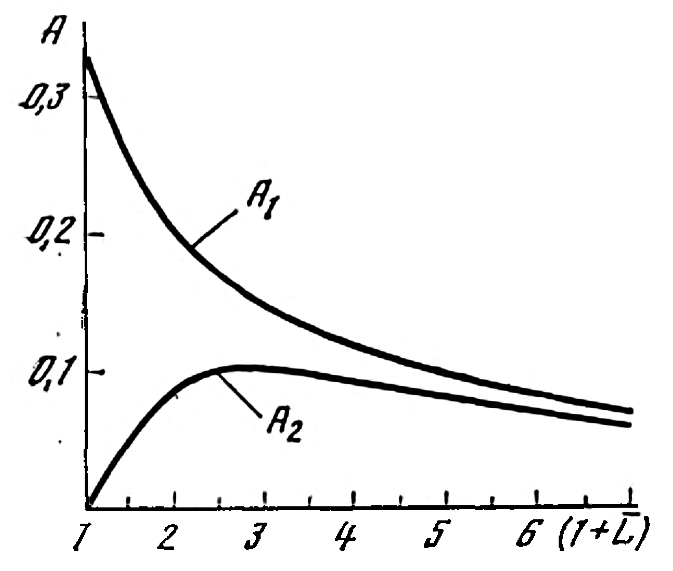
\includegraphics[width=0.45\linewidth]{figures/f4.1.png}
\end{figure}
\figblock{4.1}{Graphs of $\Delta_1$ and $\Delta_2$ as functions of $1+l$, computed from
  formulas~(4.3) and~(4.4) with $\delta = 0.5$ and $P_1(l) = 1 + \arctan l$.  The curve
  $\Delta_2$ lies everywhere below $\Delta_1$ (inequality~4.5) and satisfies $\Delta_2 = 0$
  both at $l=0$ and as $l\to\infty$, while $\Delta_1 = 0$ only as $l\to\infty$.}

Fig.\,4.1 shows the variation of $\Delta_1$ and $\Delta_2$ computed from formulas~(4.3)
and~(4.4) for $\delta = 0.5$, using the specific form of $P_1(l)$ given by formula~(3.1).
The graphs show that the convergence of curves $\Delta_1$ and $\Delta_2$ occurs somewhere
in the region $1 + l \approx 4$ and becomes increasingly complete as $l$ grows.  This
testifies to the similarity of the linear and perceptual perspective systems for distant
regions of space.  The overall behaviour of the curves also shows that $\Delta_1 \to 0$ and
$\Delta_2 \to 0$ only as $l \to \infty$, while in contrast to $\Delta_1$ the function
$\Delta_2 = 0$ already at $l = 0$.  The curve $\Delta_2$ lies everywhere below $\Delta_1$,
illustrating inequality~(4.5).

\srcpage{260}

If one recalls that the perceptual perspective system correctly transmits the numerical
characteristics of the geometric images arising in human consciousness, then the divergence
of curves $\Delta_1$ and $\Delta_2$ (especially for small~$l$) testifies to the departure of
the geometry of the linear perspective system from the geometry of visual perception.
